\pdfoutput=1
\documentclass[11pt,a4paper]{article}

% ---- Packages ----
\usepackage[utf8]{inputenc}
\usepackage[T1]{fontenc}
\usepackage{lmodern}
\usepackage{microtype}
\usepackage{amsmath,amssymb,amsthm,mathtools}
\usepackage[a4paper,margin=1in]{geometry}
\usepackage{xcolor}
\usepackage[unicode,colorlinks=true,linkcolor=blue,citecolor=blue,urlcolor=magenta]{hyperref}
\usepackage[nameinlink,capitalize]{cleveref}
\usepackage{booktabs}
\usepackage{siunitx}
\usepackage[section]{placeins}
\sisetup{group-separator={\,},detect-all}
\usepackage{pgfplots}
\pgfplotsset{compat=1.17} % arXiv-safe (slightly older than 1.18)
\usetikzlibrary{positioning,arrows.meta,shapes,calc}
\usepackage{graphicx}

% avoid overfull boxes
\setlength{\emergencystretch}{3em}

% Disable math macros inside PDF bookmarks
\pdfstringdefDisableCommands{%
  \def\gap{lambda2}%
  \def\hdeg{hdeg}%
  \def\nL{L}%
}

% ---- Theorem environments ----
\newtheorem{theorem}{Theorem}
\newtheorem{lemma}{Lemma}
\newtheorem{proposition}{Proposition}
\newtheorem{conjecture}{Conjecture}
\theoremstyle{remark}
\newtheorem*{remark}{Remark}

% ---- Macros ----
\newcommand{\nL}{\mathcal{L}}
\newcommand{\gap}{\lambda_2}
\newcommand{\hdeg}{\widehat{\deg}}

% ===== TITLE =====
\title{\textbf{Spectral Predictors for Tseitin Hardness:\\
A Physics-Motivated Exploration}\\
\large Preliminary Conjectures and Empirical Observations}

\author{\textbf{Amandine Morin}%
\footnote{Research conducted independently.}%
\footnote{No institutional affiliation.}}

\date{Revised February 2026}

\begin{document}
\maketitle

\begin{center}
\small
\textcolor{red}{\textbf{EXPLORATORY PREPRINT — NOT PEER-REVIEWED}}\\[0.5em]
\textcolor{blue}{This work presents \textbf{conjectures and preliminary observations}
on spectral predictors for proof complexity. No new theorems are proved.
Empirical validation is limited to small illustrative instances ($n \leq 80$).
This document invites discussion, testing, and critique.}
\end{center}

\begin{abstract}
We explore a physics-first viewpoint on propositional proof complexity, motivated by
Landauer's principle~\cite{Landauer1961}: information processing has an inherent physical cost.
For Tseitin contradictions over quasi-regular graphs~\cite{Tseitin1968,KrajicekBook}, we argue
that any solver must process a minimal amount of \emph{structural information} depending jointly
on local density and global connectivity.

We introduce the predictor
\[
\hdeg(G) := \frac{n}{\sqrt{1/d + 1/\gap}},
\]
where $n$ is the number of vertices, $d$ the average degree, and $\gap$ the second-smallest
eigenvalue of the normalized Laplacian~\cite{Chung1997}.
We formulate corresponding Kolmogorov-type information conjectures~\cite{LiVitanyi},
conjectural decision-tree lower bounds, and connections to Polynomial Calculus degree.

Empirically, we observe that small structural perturbations can induce sharp,
solver-dependent transitions in SAT solver behavior at fixed $(n,d)$,
notably under Watts--Strogatz rewiring.
We interpret these transitions as evidence for underlying \emph{information thresholds}
governing solver difficulty.

\medskip
\noindent\textbf{Note.} This is an exploratory preprint presenting conjectures and
preliminary empirical observations. No new theorems are proved.
\end{abstract}

\paragraph{Contributions.}
This exploratory work offers:
\begin{itemize}
  \item A physics-motivated \emph{conjectural} framework linking spectral structure
        to proof complexity for Tseitin formulas;
  \item A structural predictor $\hdeg(G)$ combining local density and global connectivity;
  \item Empirical evidence of a \emph{structural phase transition} in SAT solver behavior
        under small graph perturbations at fixed $(n,d)$;
  \item A preliminary connection between these transitions and information-theoretic
        interpretations of solver complexity;
  \item A roadmap of conjectures linking spectral graph theory, decision-tree complexity,
        Polynomial Calculus, and Kolmogorov complexity.
\end{itemize}
\textbf{No new theorems are proved.}

% ============================
\section{Introduction}

The cost of distinguishing SAT from UNSAT is fundamentally informational.
A solver must extract, manipulate, and retain a minimal volume of structural information
about the instance. Following Landauer's principle~\cite{Landauer1961}, we take seriously
the idea that this informational cost has a structural footprint in the input.

Tseitin contradictions~\cite{Tseitin1968,KrajicekBook} are among the canonical hard families
in propositional proof complexity. They encode parity constraints on a graph $G$ and are
unsatisfiable exactly when the total charge is odd. On expander graphs, Tseitin formulas
yield strong lower bounds in Resolution~\cite{BenSassonWigderson2001} and algebraic systems
such as Polynomial Calculus (PC)~\cite{Razborov1998}.

Meanwhile, spectral graph theory~\cite{Chung1997,HooryLinialWigderson} provides a robust way
to quantify connectivity via the spectrum of the normalized Laplacian, with the spectral gap
$\gap$ tightly related to edge expansion and mixing.

In this preprint we propose a structural predictor,
\[
\hdeg(G) = \frac{n}{\sqrt{1/d + 1/\gap}},
\]
combining local density ($d$) and global connectivity ($\gap$) in a harmonic fashion.
We conjecture that $\hdeg(G)$ approximates the minimal information budget that any
reasoning process must handle to refute $\mathrm{Tseitin}(G,\chi)$.
We phrase this in time-bounded Kolmogorov terms~\cite{LiVitanyi} and
as conjectured lower bounds in decision-tree and algebraic proof models.

Our goal here is not to present a complete lower-bound proof, but to propose a coherent
structural scale that can be probed both analytically and empirically, and which appears
to interpolate naturally between known behaviors on cycles, grids, expanders and dense graphs.

Even when the degree is fixed, the global geometry of the constraint graph can vary
significantly depending on the generation model, as illustrated in
Figure~\ref{fig:graph_models_contrast}.

\begin{figure}[ht]
  \centering
  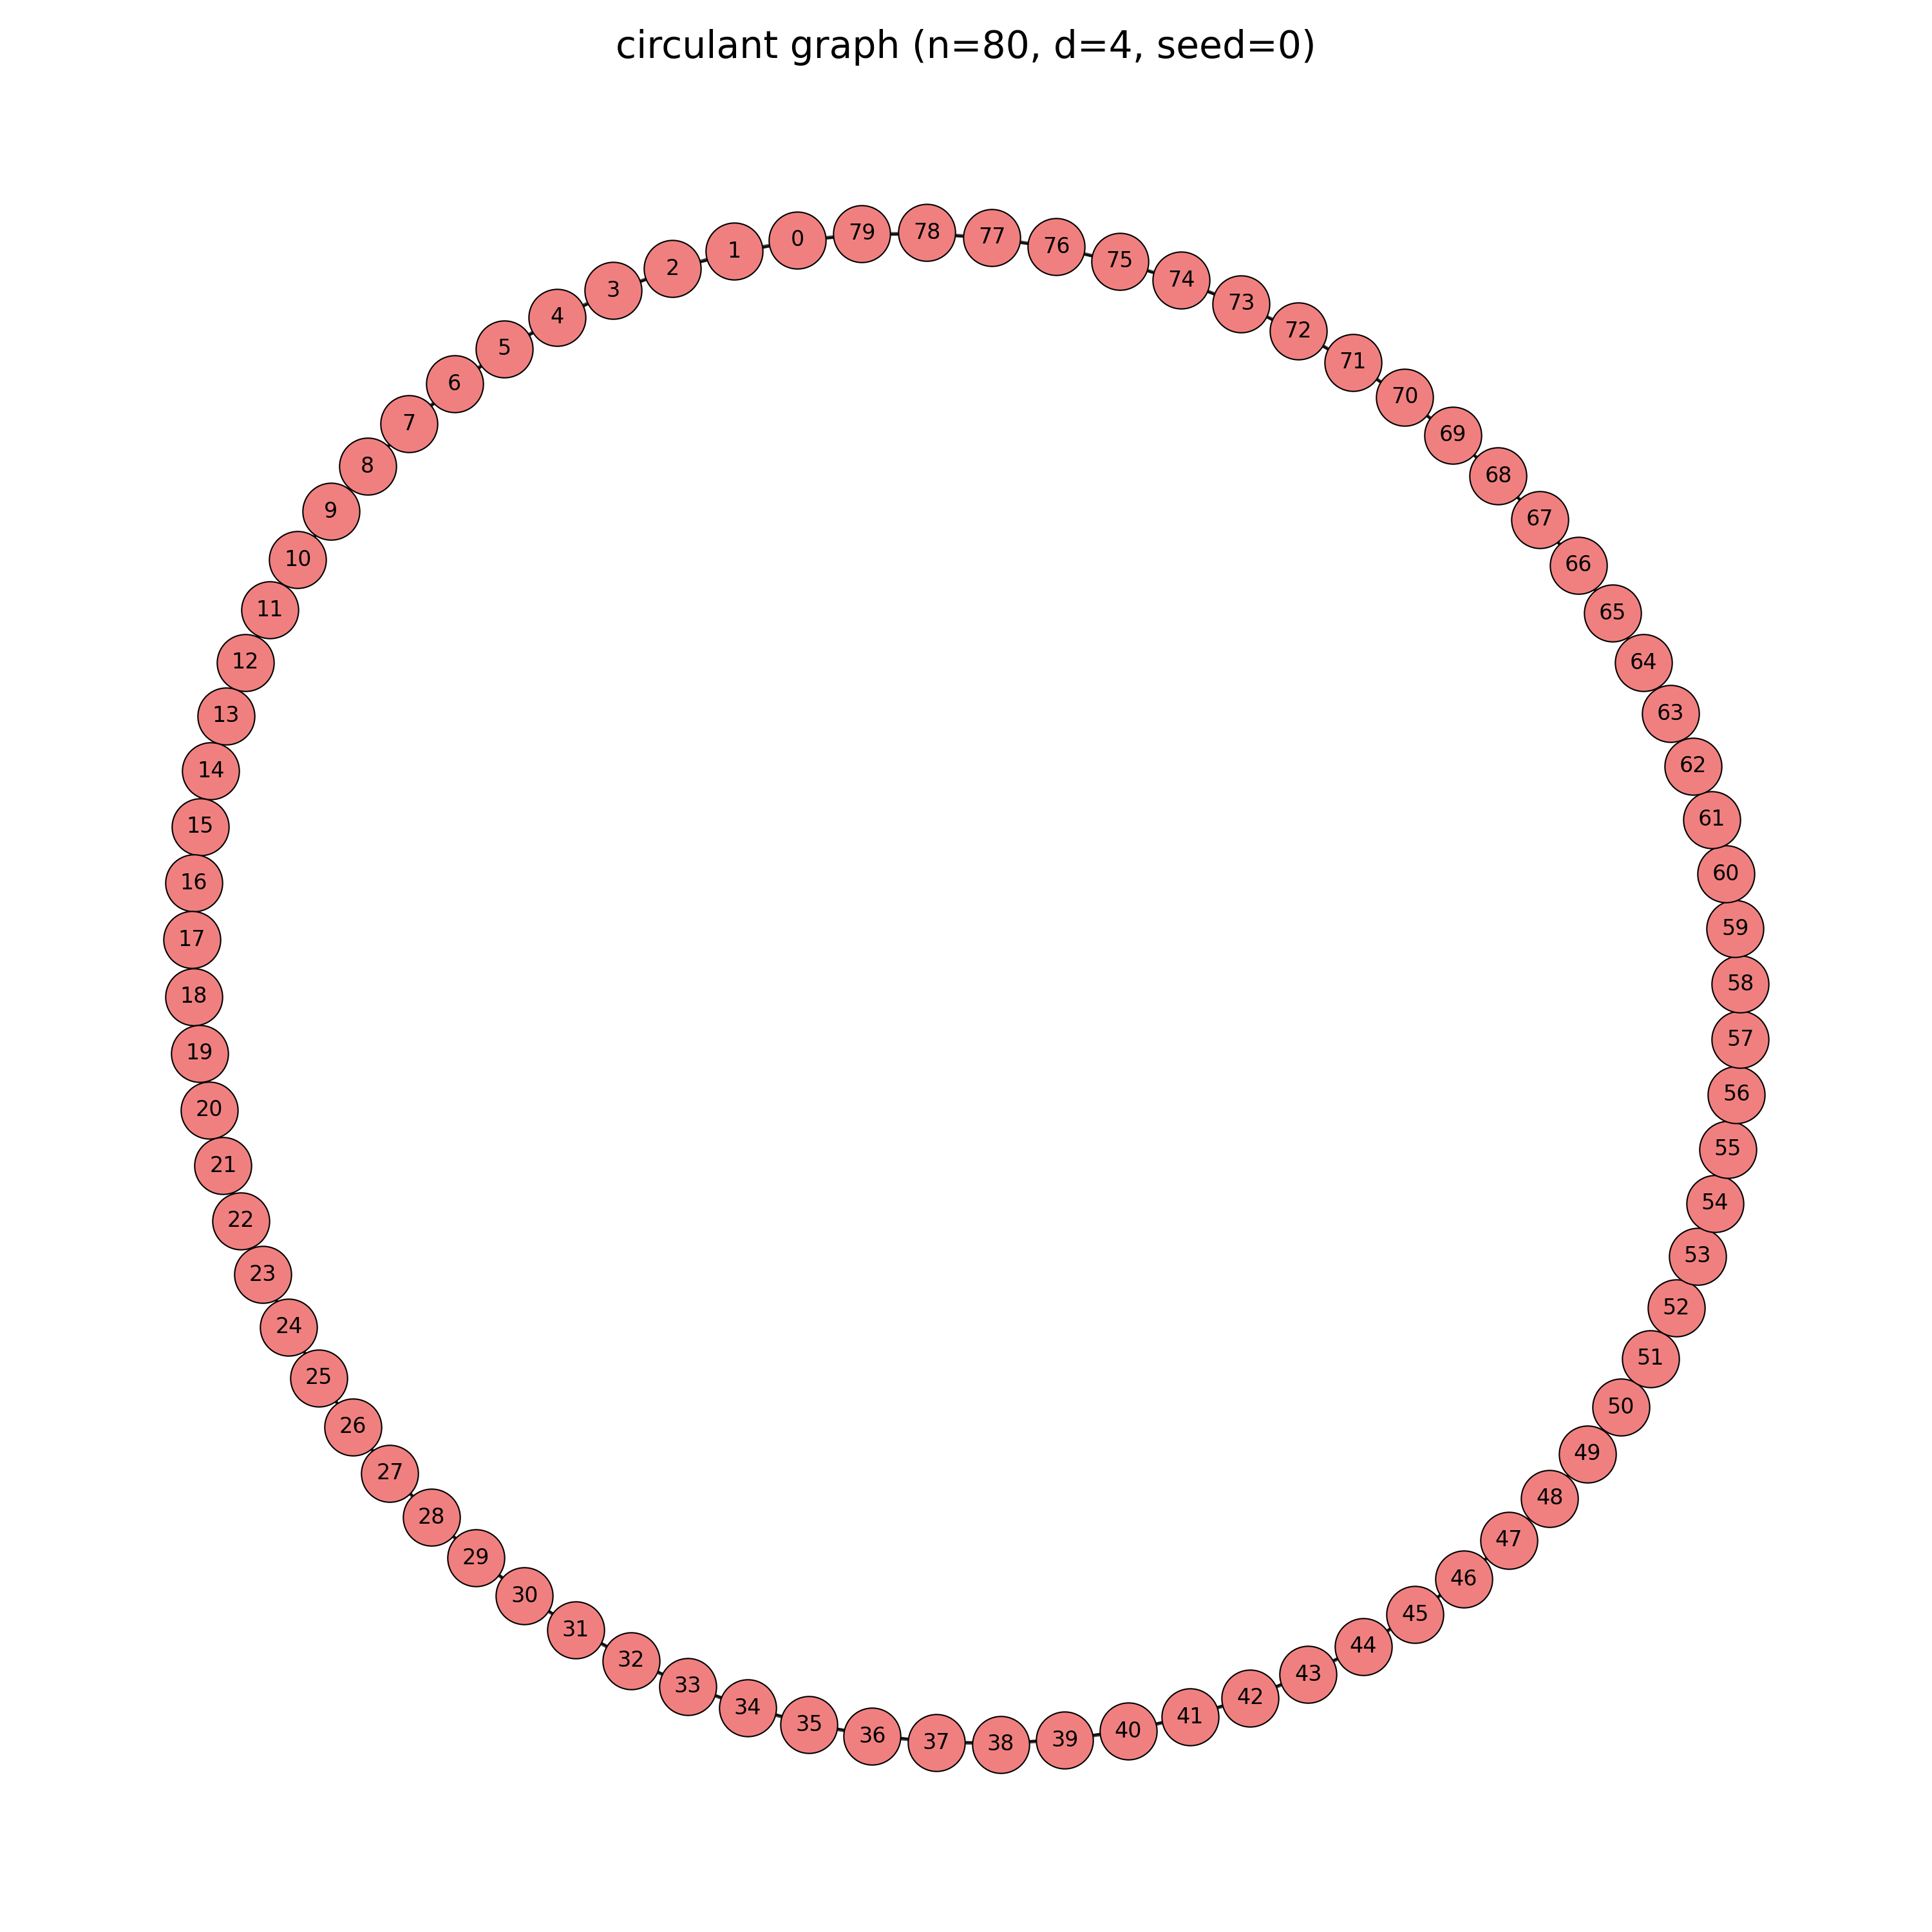
\includegraphics[width=0.48\linewidth]{../figures/circulant_n80_d4_s0.png}\hfill
  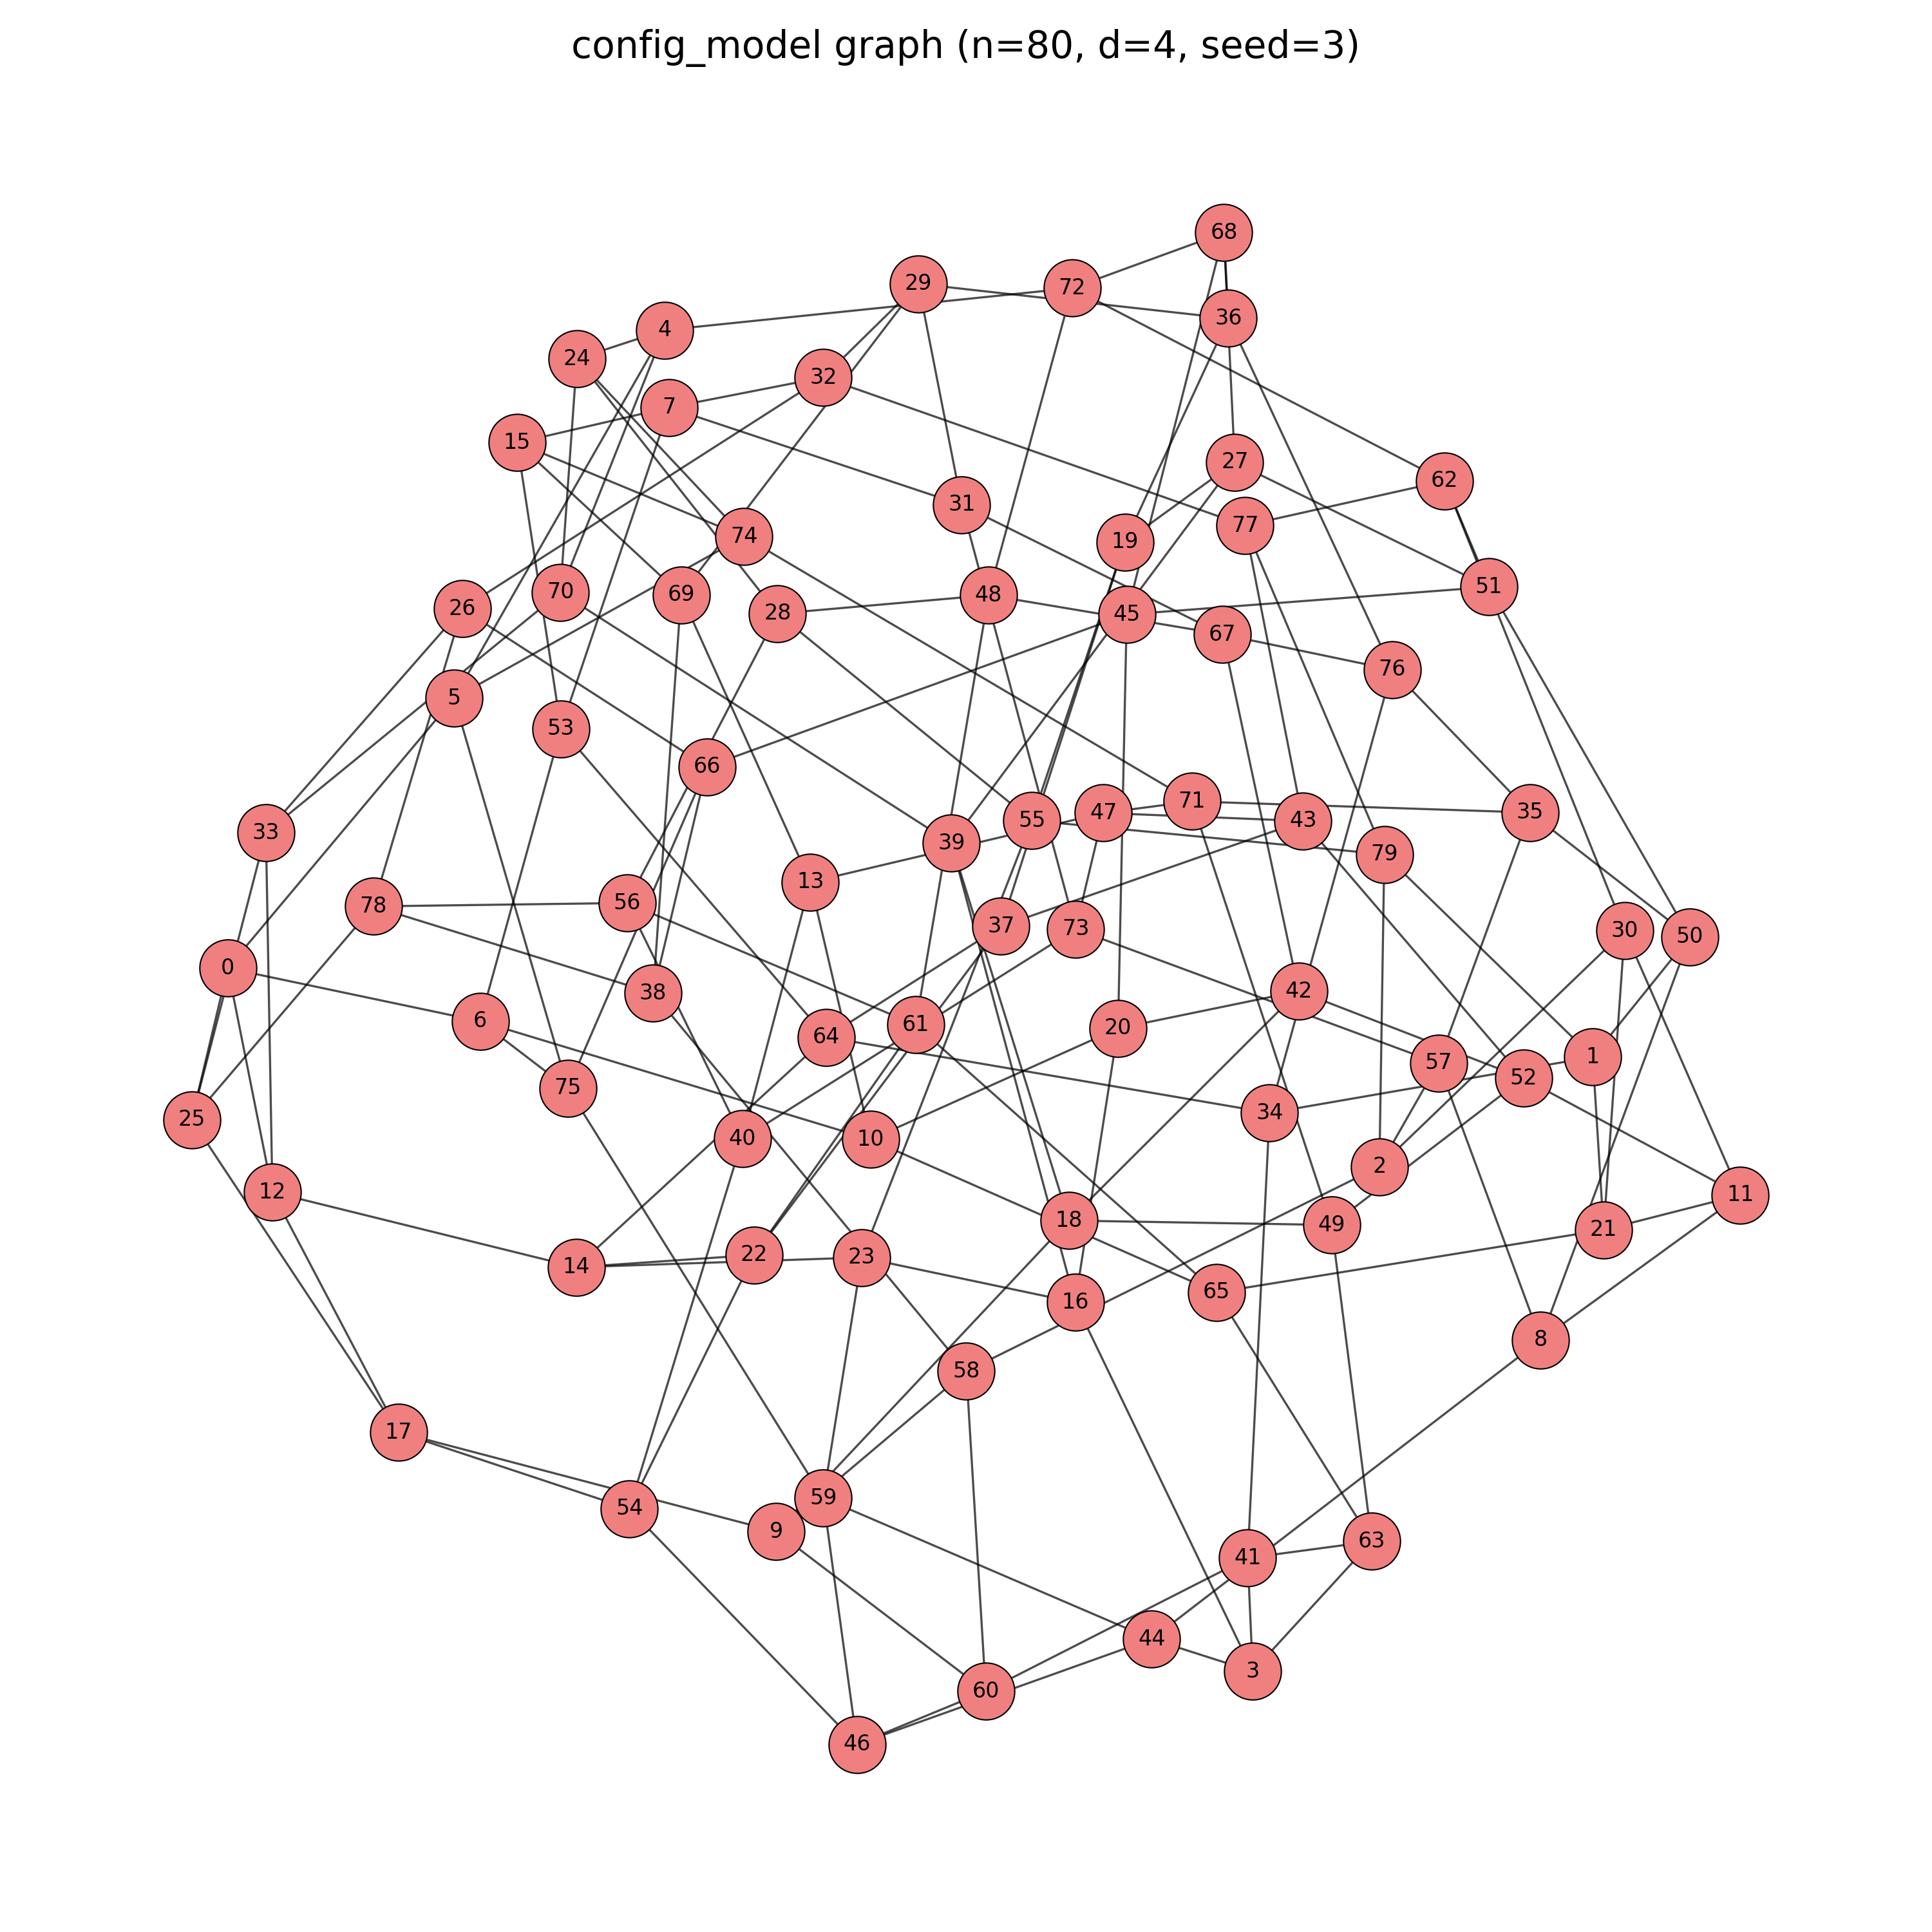
\includegraphics[width=0.48\linewidth]{../figures/config_n80_d4_s3.png}
  \caption{
  Degree-regular graphs with identical parameters ($n=80$, $d=4$) generated using two
  different models.
  \textbf{Left:} circulant graph (highly symmetric, homogeneous geometry).
  \textbf{Right:} configuration-model graph (irregular geometry with local bottlenecks).
  Despite identical degree sequences, the resulting structures differ substantially at the geometric level.
  }
  \label{fig:graph_models_contrast}
\end{figure}
\FloatBarrier

While the spectral predictor $\hdeg(G)$ provides a guiding theoretical hypothesis,
our experimental results primarily highlight strong structural sensitivity phenomena.
In particular, we observe that very small perturbations in graph structure can induce
abrupt transitions in solver behavior, suggesting the existence of underlying
information thresholds.

% ============================
\section{Graphs, spectrum, and conventions}

Let $G=(V,E)$ be a simple graph with $|V|=n$ and average degree $d$.
The normalized Laplacian is
\[
\nL = I - D^{-1/2} A D^{-1/2},
\]
with eigenvalues
\[
0 = \lambda_1 \le \gap \le \cdots \le \lambda_n \le 2,
\]
where $\gap$ is the second-smallest eigenvalue (the spectral gap)~\cite{Chung1997}.

\begin{remark}[Cheeger inequality]
Let $\phi(G)$ denote edge conductance.
Cheeger-type inequalities for the normalized Laplacian~\cite{Chung1997} give
\[
\frac{\phi(G)^2}{2} \le \gap \le 2\phi(G),
\]
supporting the use of $\gap$ as a proxy for expansion.
\end{remark}

We focus on quasi-regular families (bounded ratio between maximum and minimum degrees),
and we view $G$ as the constraint graph of a Tseitin formula~\cite{Tseitin1968,KrajicekBook}.

% ============================
\section{MPCC and Kolmogorov formulation}

We now phrase the Minimal Proof Compression Conjecture (MPCC) and a
Kolmogorov-based variant.

\begin{conjecture}[MPCC]\label{conj:mpcc}
For any quasi-regular family of graphs, any solver deciding $\mathrm{Tseitin}(G,\chi)$
must process at least
\[
c\cdot \frac{n}{\sqrt{1/d + 1/\gap}}
\]
bits of structural information about $G$, for some constant $c>0$, robust under
preprocessing and natural re-encodings.
\end{conjecture}

\paragraph{Kolmogorov formulation.}
Following Li--Vitányi~\cite{LiVitanyi}, let $K^t$ denote time-bounded Kolmogorov
complexity with side information. For a canonical encoding $\mathrm{enc}(G)$, set
\[
K^t(G \mid (n,d,\gap))
=\min\{|p| : U(p,(n,d,\gap)) = \mathrm{enc}(G) \text{ in time } \le t(|G|)\}.
\]

\begin{conjecture}[Kolmogorov--MPCC]\label{conj:kmpcc}
There exist $c>0$ and a polynomial $t(\cdot)$ such that for all quasi-regular graphs~$G$,
\[
K^t(G \mid (n,d,\gap))
\;\ge\;
c \cdot \frac{n}{\sqrt{1/d + 1/\gap}} - o(n).
\]
\end{conjecture}

% ============================
\section{Decision-tree lower bounds}

We informally sketch a decision-tree model for refuting Tseitin contradictions and
formulate our lower-bound claims as conjectures, since a fully detailed proof is not
included in this preprint.

Let $\mathrm{R}_0^{\mathrm{DT}}(G)$ denote the zero-error randomized decision-tree
complexity of refuting $\mathrm{Tseitin}(G,\chi)$, where each query requests local
information about edges and incident constraints.

\begin{conjecture}[DT lower bound for $d=O(1)$]\label{conj:dt}
For any bounded-degree quasi-regular graph $G$, there exists $c>0$ such that
\[
\mathrm{R}_0^{\mathrm{DT}}(G) \;\ge\; c\, n\sqrt{\gap}.
\]
\end{conjecture}

\begin{conjecture}[Harmonic-bound template]\label{conj:harm}
For any quasi-regular graph $G$, there exists $c>0$ such that
\[
\mathrm{R}_0^{\mathrm{DT}}(G)
\;\ge\;
c \cdot \frac{n}{\sqrt{1/d + 1/\gap}}.
\]
\end{conjecture}

These conjectures are motivated by Yao-style arguments and the behavior of
expander graphs~\cite{HooryLinialWigderson}.

% ============================
\section{Polynomial Calculus connections}

Polynomial Calculus (PC) is an algebraic proof system where propositional formulas
are translated into polynomial equations over a field and refutations proceed by
algebraic derivations~\cite{Razborov1998,KrajicekBook}. For Tseitin contradictions
over expanders and fields of characteristic not equal to $2$, Razborov~\cite{Razborov1998}
proved linear lower bounds on PC degree.

These results fit the qualitative picture suggested by $\hdeg(G)$: stronger expansion
implies higher degree, and thus higher algebraic complexity.

\begin{conjecture}[PC-degree $\Rightarrow$ touch complexity]\label{conj:pc-touch}
If $\deg_{\mathsf{PC}}(\mathrm{Tseitin}(G)) \ge r$ then
\[
\mathrm{Touch}_{\mathsf{PC}}(G) \;\ge\; c r
\]
for some absolute constant $c>0$, where $\mathrm{Touch}_{\mathsf{PC}}(G)$ is a
suitable measure of how many constraint occurrences any PC derivation must ``touch''.
\end{conjecture}

We expect $\mathrm{Touch}_{\mathsf{PC}}(G)$ to scale with $\hdeg(G)$, linking
PC-degree lower bounds to the MPCC perspective.

% ============================
\section{Calibrating the predictor $\hdeg(G)$}

We define
\[
\hdeg(G) := \frac{n}{\sqrt{1/d + 1/\gap}}.
\]

This form matches natural scales on standard graph families~\cite{Chung1997,HooryLinialWigderson}:

\begin{center}
\renewcommand{\arraystretch}{1.05}\small
\begin{tabular}{lcccc}
\toprule
Family          & $d$   & $\gap$           & $\hdeg(G)$        & Comment        \\
\midrule
Cycle $C_n$     & 2     & $\Theta(1/n^2)$ & $\Theta(1)$       & 1-D weak       \\
Grid $m\times m$& $O(1)$& $\Theta(1/n)$   & $\Theta(\sqrt{n})$& 2-D medium     \\
Expander        & $O(1)$& $\Theta(1)$     & $\Theta(n)$       & strong         \\
Complete $K_n$  & $n$   & 1               & $\Theta(n)$       & dense          \\
\bottomrule
\end{tabular}
\end{center}

% ============================
\section{Empirical Results}

We test the alignment between $\hdeg(G)$ and practical SAT difficulty for Tseitin CNFs.
Families include cycles $C_n$, grids, complete bipartite graphs, and random regular graphs.
CNFs are generated by constructing $G$ and encoding XOR constraints at each vertex into
3-CNF using auxiliary variables.

We present controlled experiments investigating the impact of graph structure
on solver behavior, as well as preliminary evidence relating this behavior
to the spectral predictor $\hdeg(G)$.

% ============================
\subsection{Experimental pipeline and structure dependence}

We use a reproducible C++ pipeline in which each instance is fully determined by
$(n,d,\texttt{seed},\texttt{graph\_mode},p)$.
The pipeline generates the graph, builds the corresponding Tseitin CNF,
computes a byte-level hash of the DIMACS file (\texttt{cnf\_hash}),
and runs a SAT solver under fixed resource limits.

We evaluate two CDCL solvers:
\begin{itemize}
  \item \textbf{Kissat} (modern high-performance solver),
  \item \textbf{MiniSat} (baseline reference solver).
\end{itemize}

All runs use a \SI{60}{\second} wall-clock timeout.
Each configuration is evaluated over 5 independent seeds.

At fixed size $n=80$ and degree $d=4$, we observe strong structure dependence
even when $(n,d)$ are held constant.
In particular, graph generation models with identical degree sequences can yield
dramatically different solver behavior.

% ============================
\subsection{Watts--Strogatz transition}

We study $d$-regular graphs generated using the Watts--Strogatz rewiring model,
with rewiring probability
\[
p \in \{0, 0.01, 0.02, 0.05\}.
\]

All instances correspond to Tseitin contradictions and are UNSAT by construction.

\paragraph{Observed transition.}

We observe a sharp transition in solver behavior, which we refer to as a
\emph{structural phase transition}.

For Kissat:
\begin{itemize}
  \item $p=0$: easy regime (median \SI{22}{\milli\second})
  \item $p=0.01$: heavy-tailed regime (median \SI{6305}{\milli\second})
  \item $p \ge 0.02$: all runs timeout
\end{itemize}

For MiniSat:
\begin{itemize}
  \item $p=0$: easy regime (median \SI{48}{\milli\second})
  \item $p \ge 0.01$: all runs timeout
\end{itemize}

The abruptness of the transition, occurring between $p=0.01$ and $p=0.02$,
suggests a threshold phenomenon rather than a smooth degradation.

\paragraph{Interpretation.}

These results indicate that small structural perturbations can dramatically alter
the effective search landscape of CDCL solvers.

The shift in transition threshold between MiniSat and Kissat suggests that
this phenomenon depends not only on instance structure, but also on the interaction
between graph geometry and solver heuristics.

In particular, the heavy-tailed regime observed for Kissat at $p=0.01$
suggests the presence of an intermediate phase in which instances remain solvable,
but require highly variable amounts of computational effort.

\paragraph{Relation to the spectral predictor.}

Although $n$ and $d$ are fixed, rewiring significantly alters the global structure
of the graph, likely affecting expansion and the spectral gap $\gap$.

While these results are consistent with the hypothesis that $\hdeg(G)$ captures
structural hardness, we do not yet compute $\gap$ for these instances.
Establishing a direct quantitative link between $\hdeg(G)$ and the observed transition
remains an important direction for future work.

% ============================
\subsection{Runtime distributions}

\begin{figure}[h]
\centering
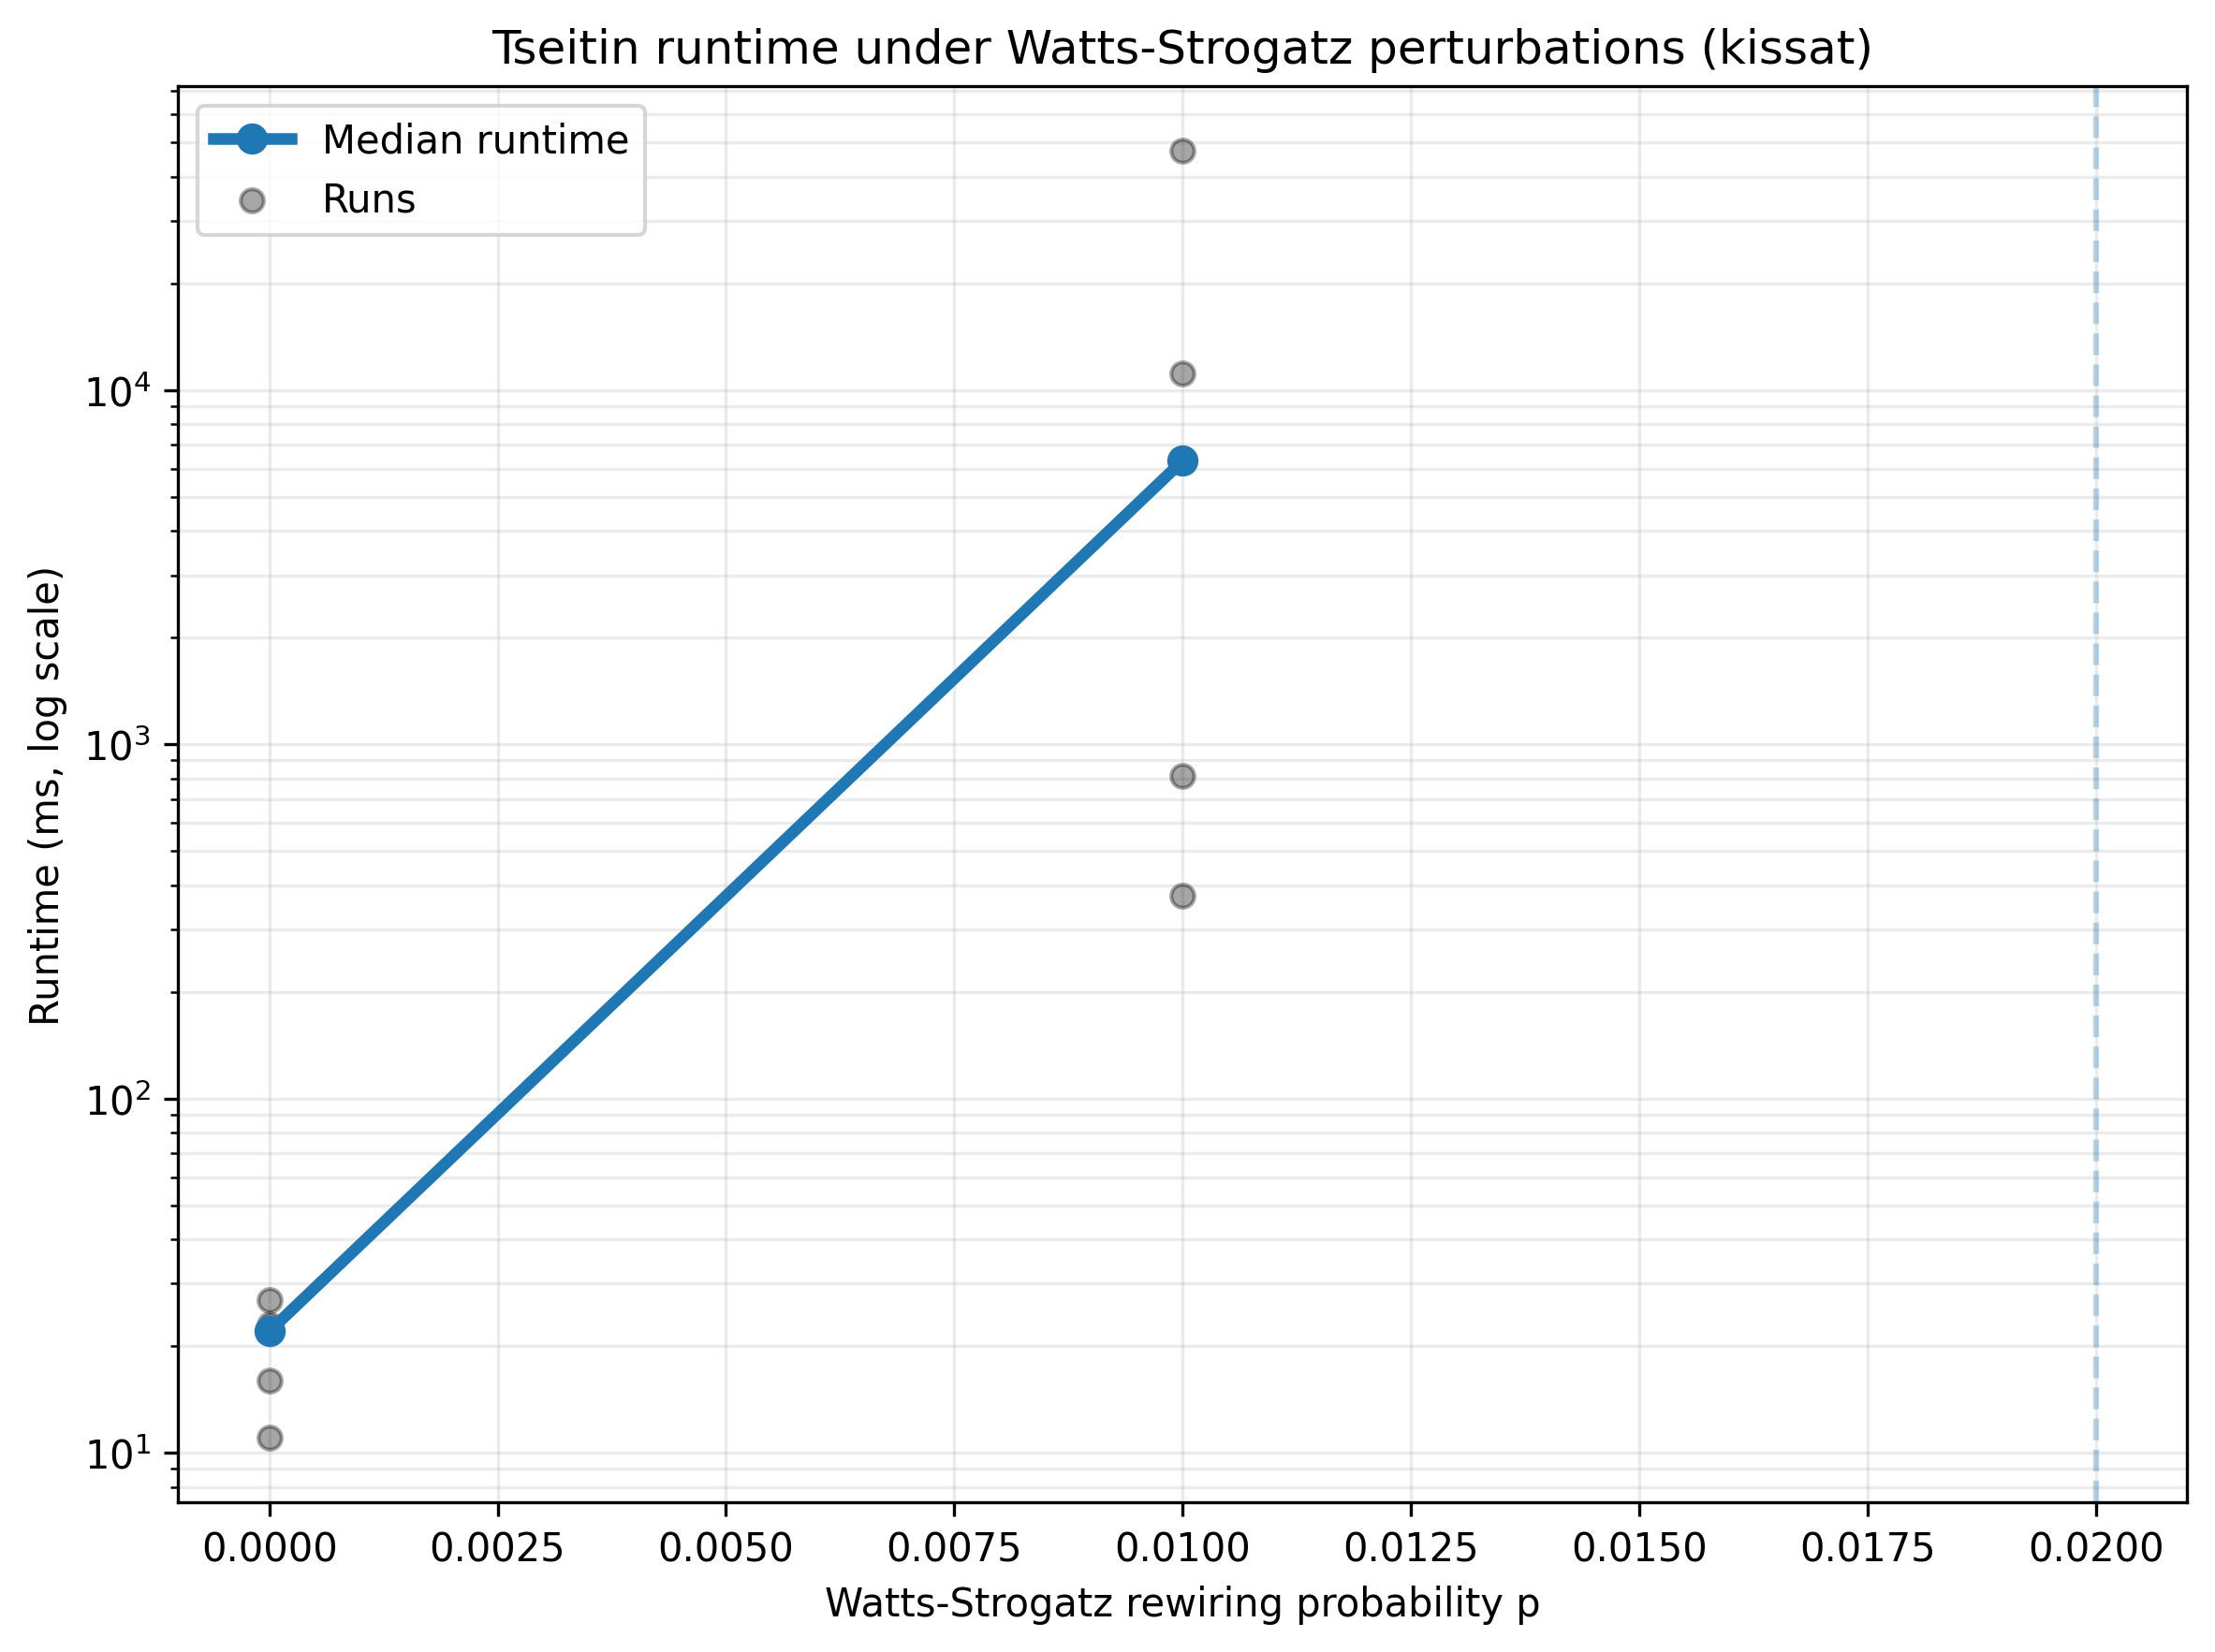
\includegraphics[width=0.8\linewidth]{../figures/ws_runtime_kissat_clean.png}
\caption{Kissat runtimes under Watts--Strogatz perturbations.
Each point corresponds to one seed; the blue curve shows the median.
A sharp increase appears at $p=0.01$, followed by systematic timeout.}
\label{fig:ws_kissat_runtime}
\end{figure}
\FloatBarrier

\begin{figure}[h]
\centering
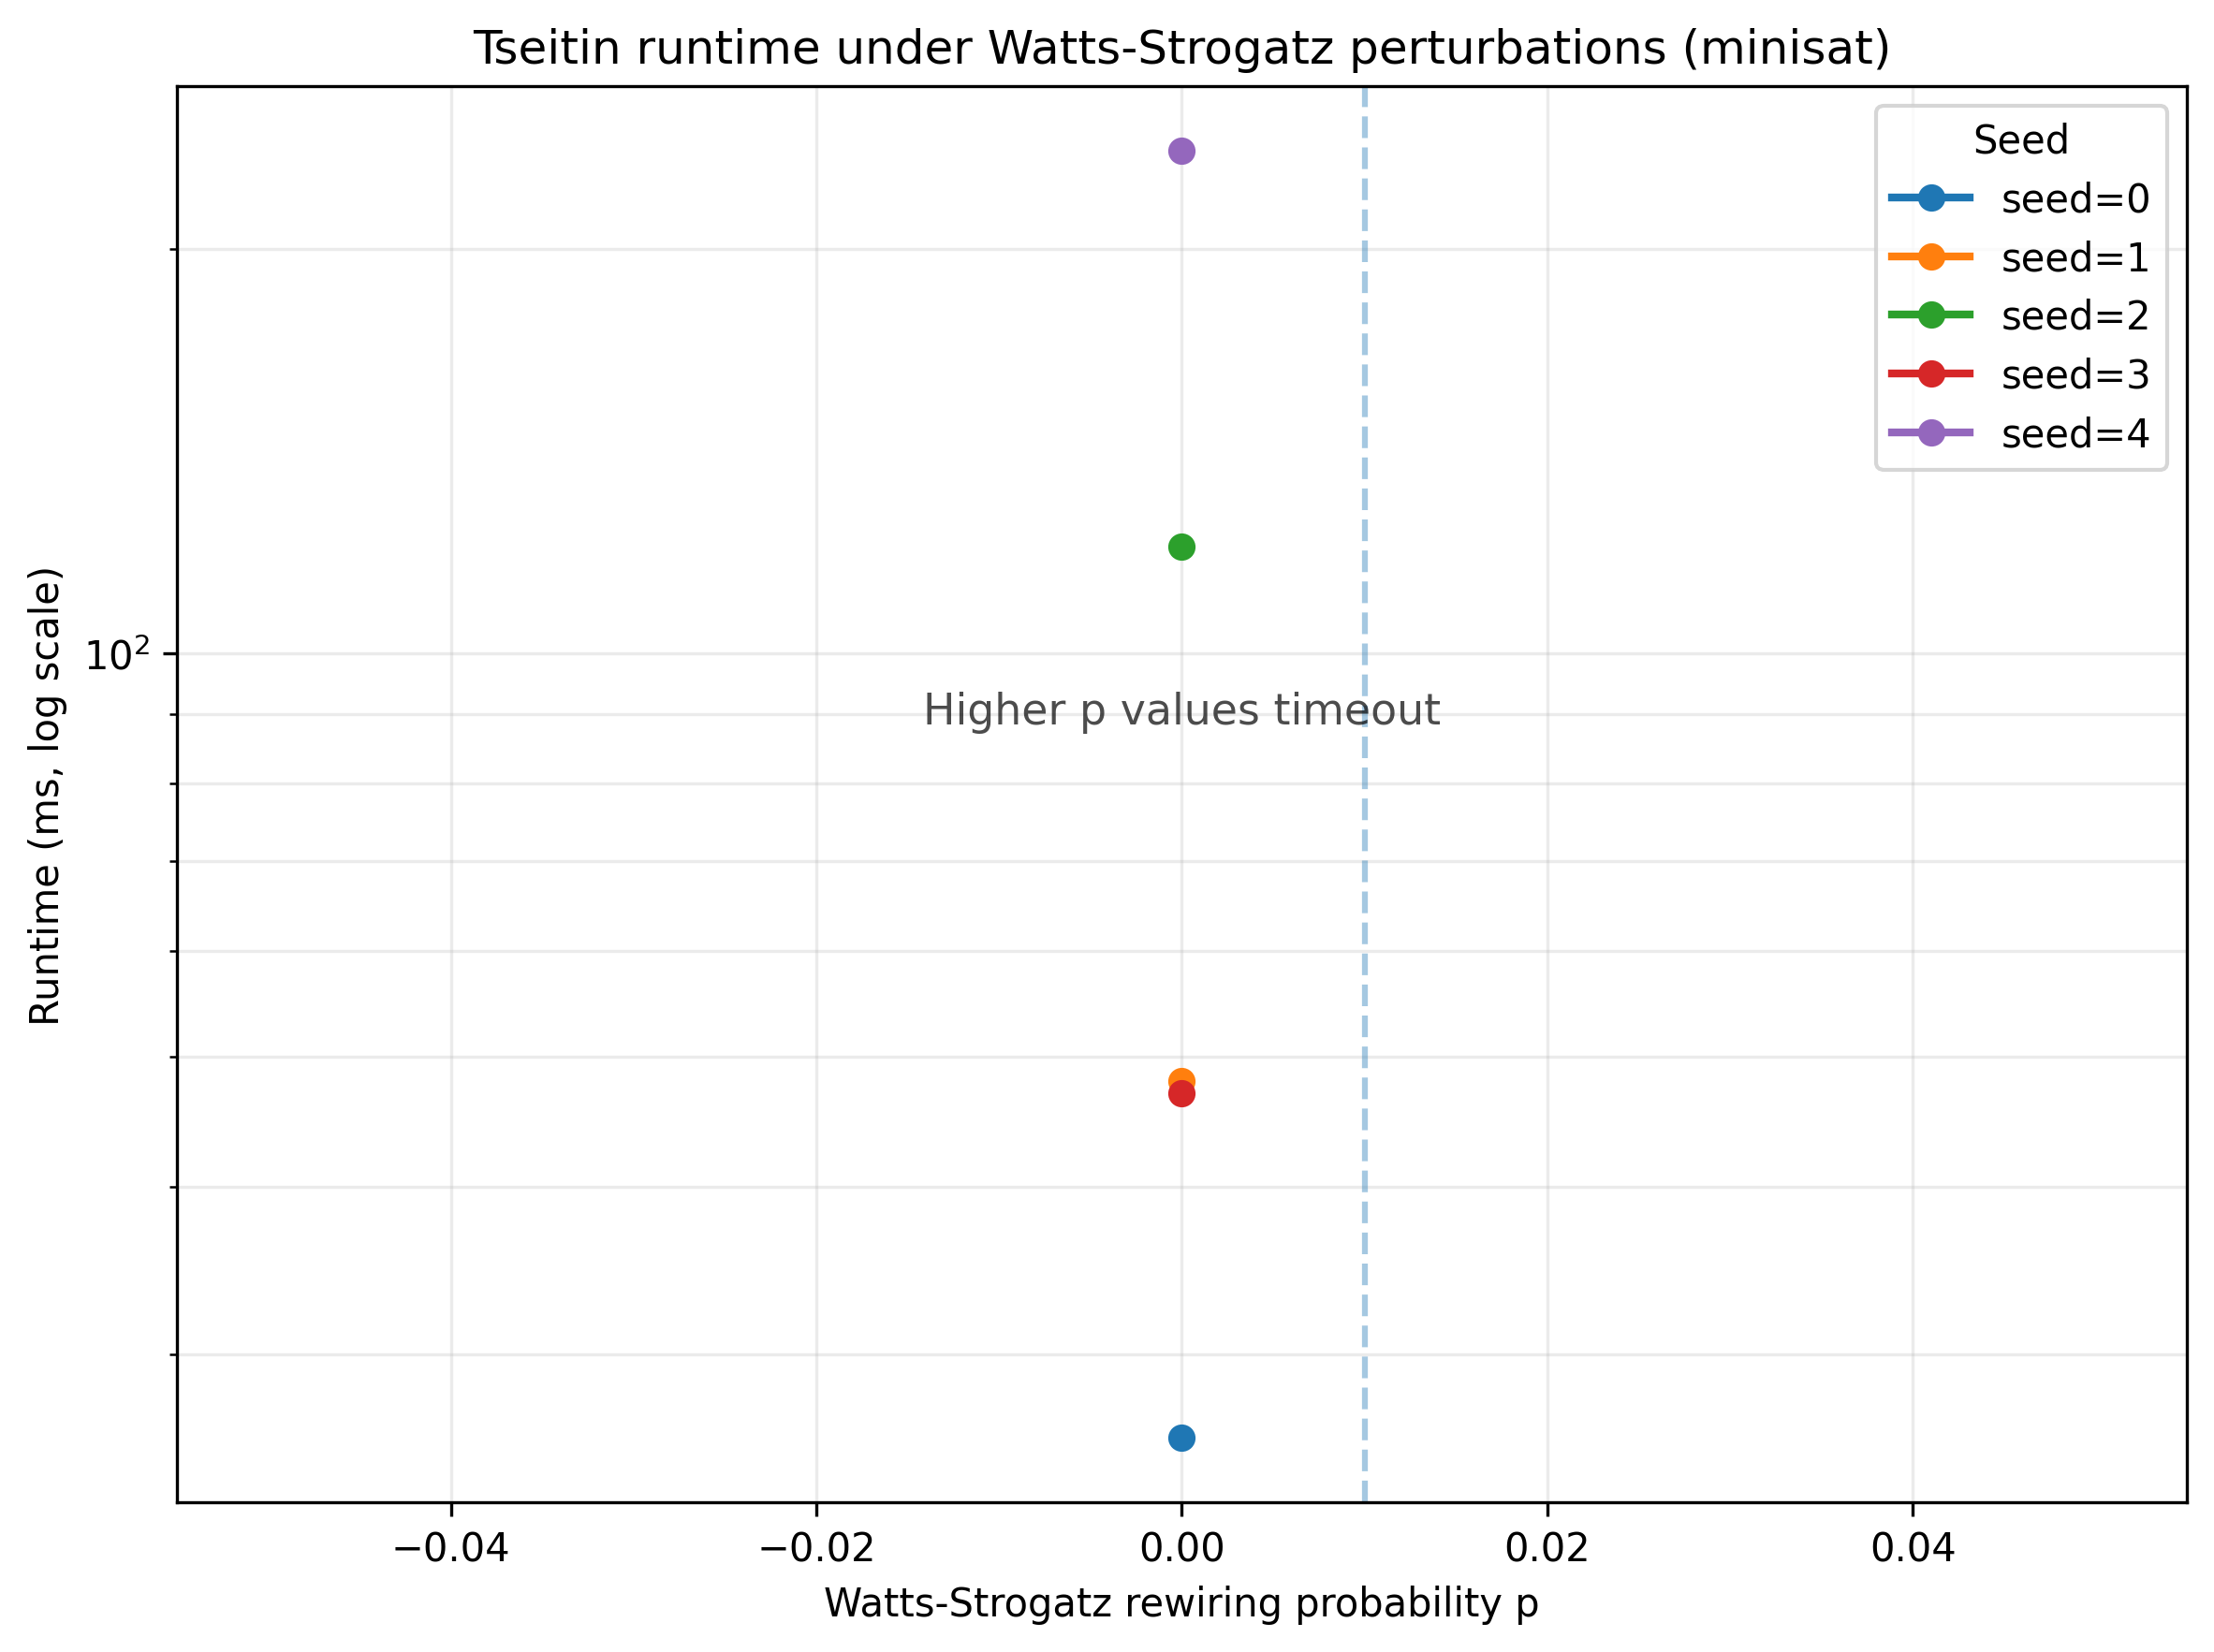
\includegraphics[width=0.8\linewidth]{../figures/ws_runtime_minisat_clean.png}
\caption{MiniSat runtimes for the same experiment.
The transition occurs earlier, with immediate timeout at $p=0.01$.}
\label{fig:ws_minisat_runtime}
\end{figure}
\FloatBarrier

\begin{figure}[h]
\centering
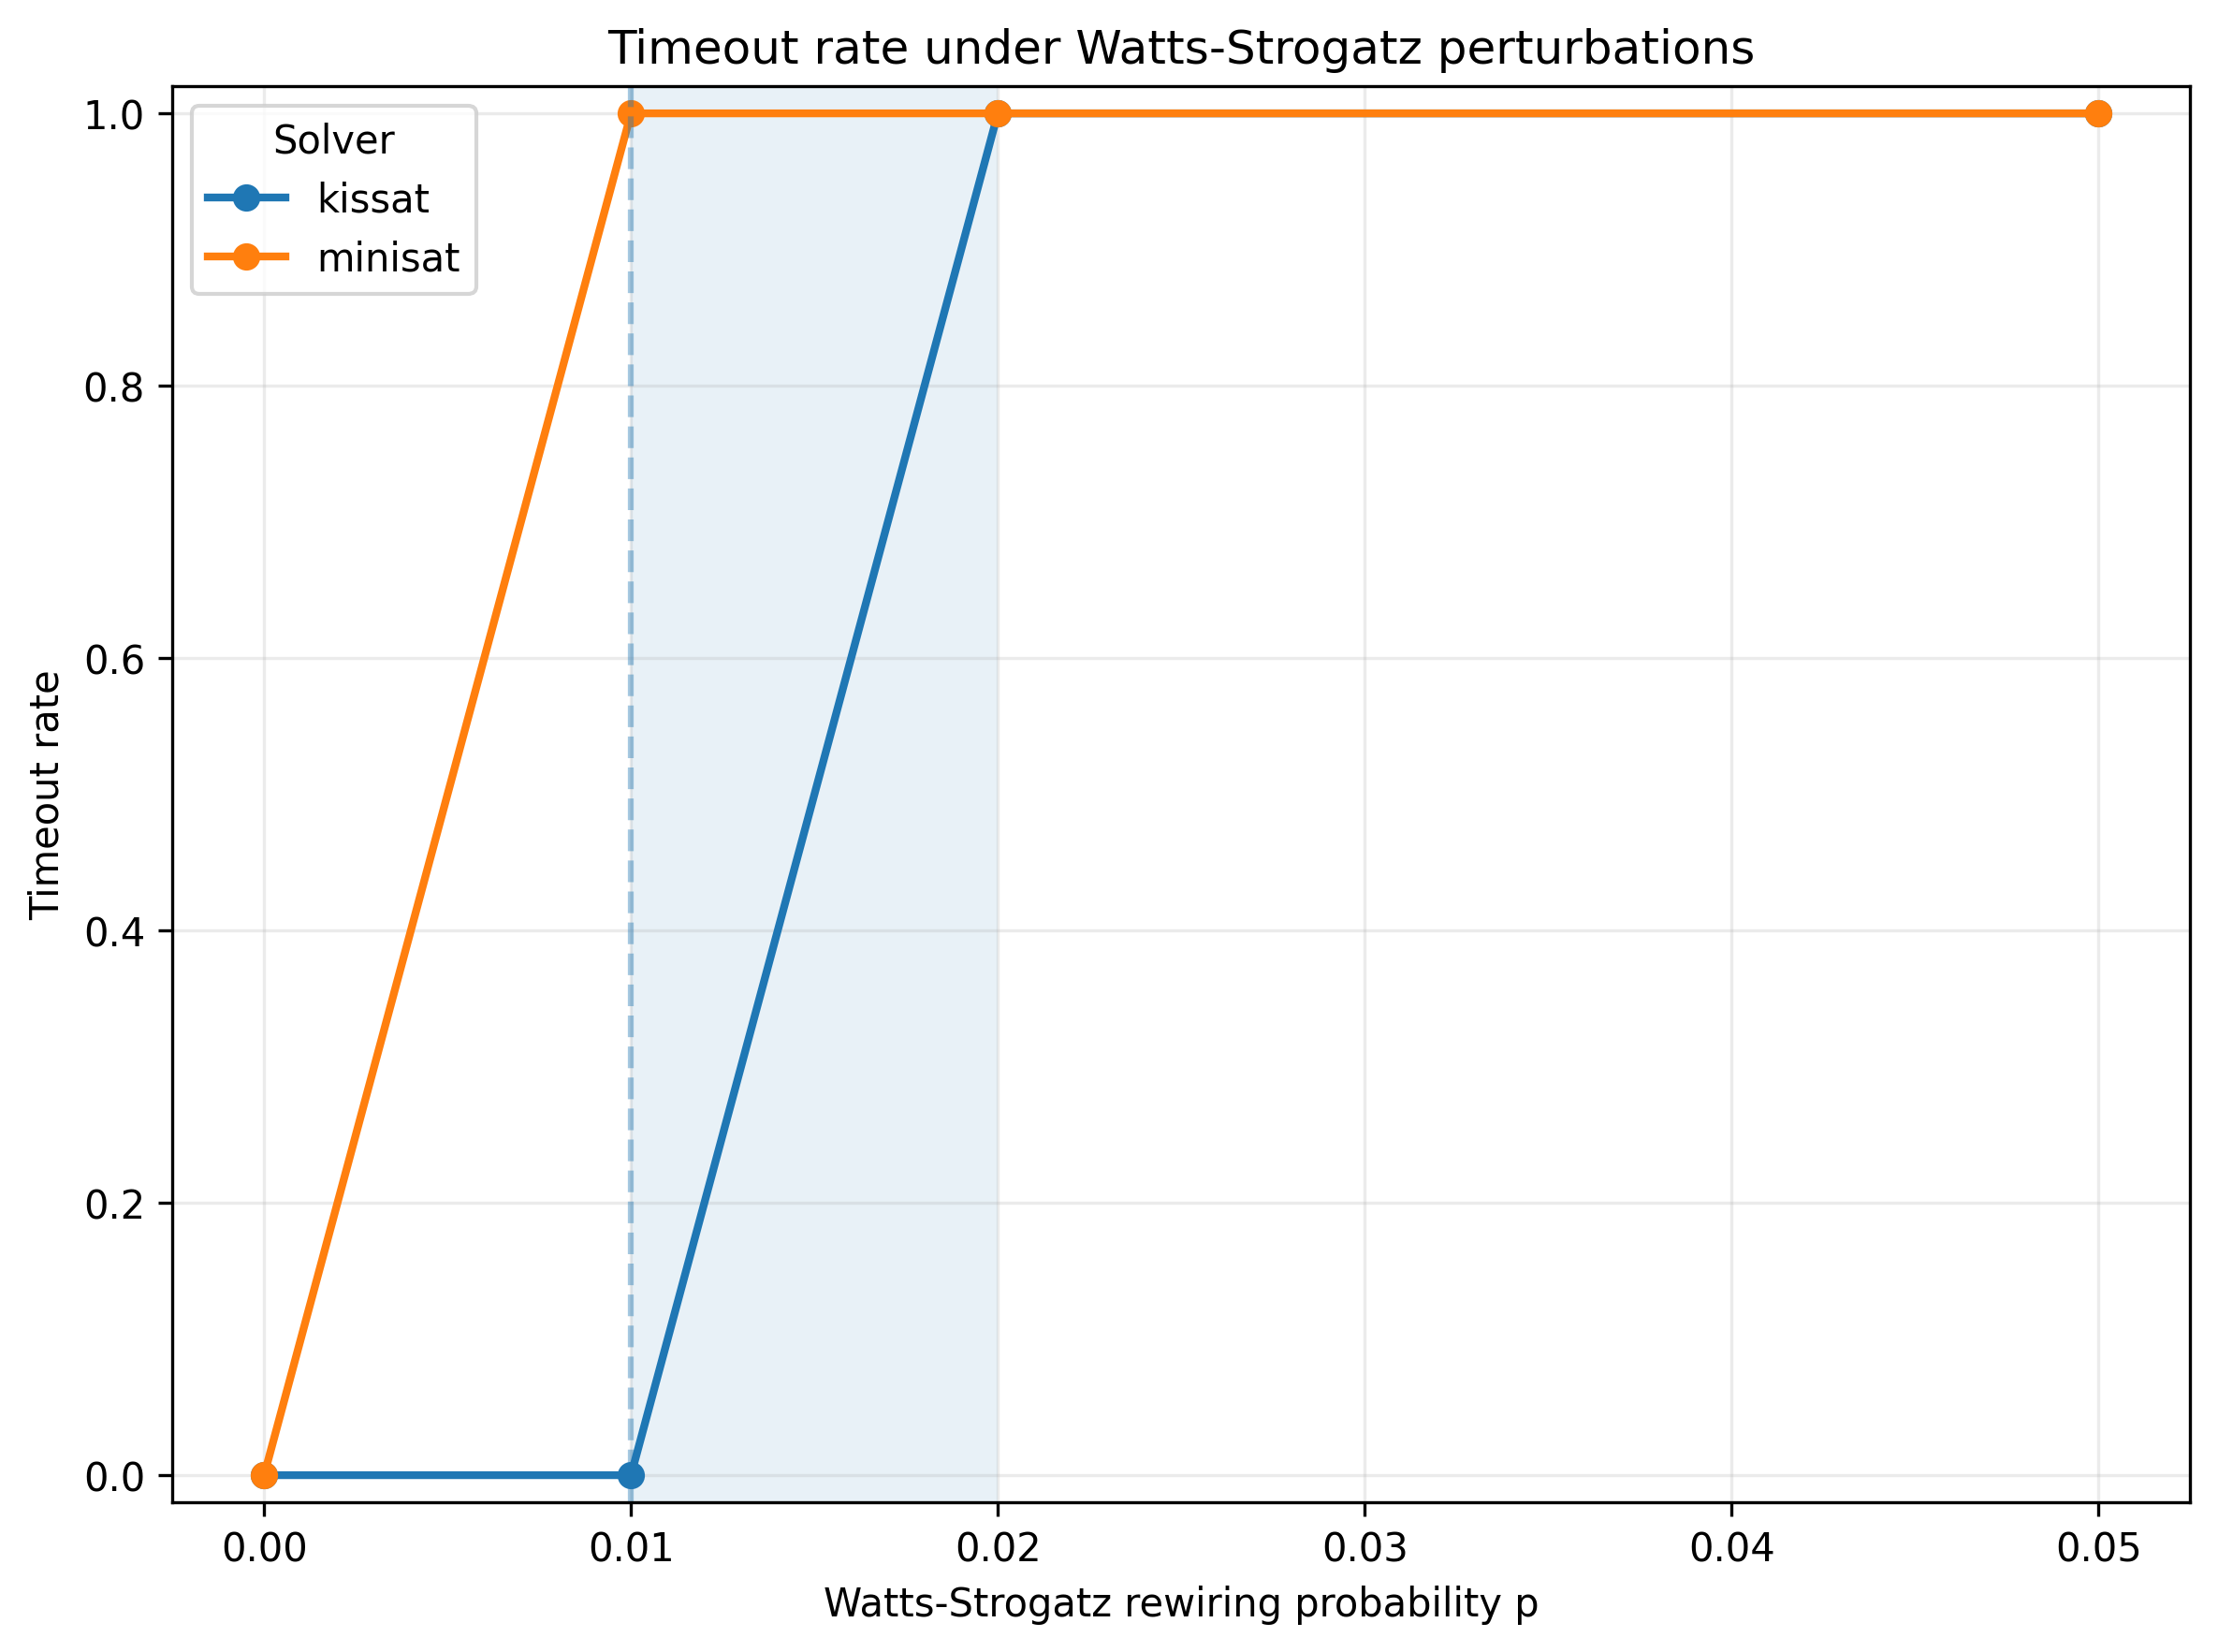
\includegraphics[width=0.8\linewidth]{../figures/ws_timeout_rate_multiseed.png}
\caption{Timeout rate as a function of rewiring probability $p$.
MiniSat reaches full timeout at $p=0.01$, whereas Kissat does so at $p=0.02$.}
\label{fig:ws_timeout_multiseed}
\end{figure}
\FloatBarrier

% ============================
\subsection{Spectral predictor vs runtime}

We compare $\hdeg(G)$ with observed solver runtimes on small benchmark families.

\begin{figure}[h]
\centering
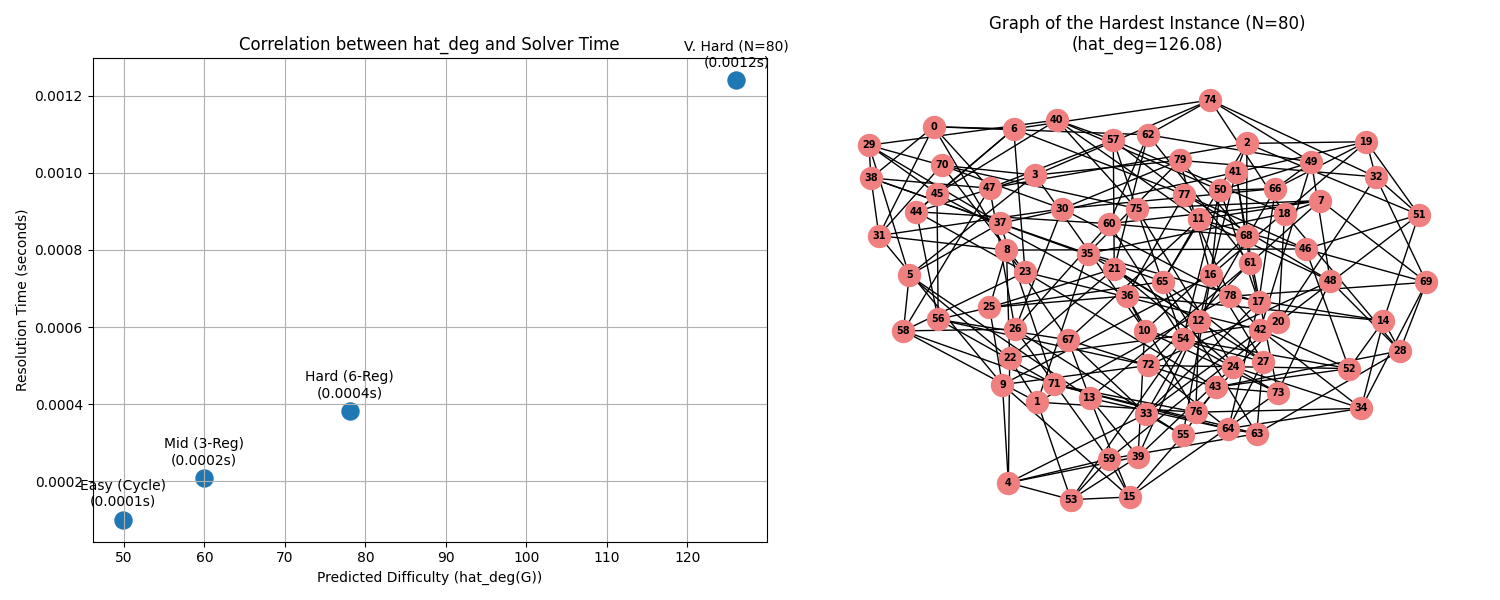
\includegraphics[width=0.8\linewidth]{../figures/tseitin_complexity_analysis.png}
\caption{Correlation between $\hdeg(G)$ and solver runtime.
Higher $\hdeg(G)$ values tend to correspond to harder instances.}
\label{fig:hdeg_correlation}
\end{figure}
\FloatBarrier

These results suggest that $\hdeg(G)$ captures a meaningful structural component
of practical SAT difficulty, although further large-scale validation is required.

% ============================
\section{Discussion: Structural Phase Transition and Information Thresholds}

The observed transition under Watts--Strogatz perturbations suggests the existence
of structural thresholds governing solver behavior.

In highly regular graphs ($p=0$), the structure appears compressible and efficiently
exploitable by CDCL heuristics.
Introducing a small amount of randomness disrupts this structure,
leading to a sharp increase in computational effort.

This behavior is consistent with the intuition underlying the MPCC conjecture:
solvers must process a minimal amount of structural information before deriving a contradiction.

The existence of solver-dependent thresholds further suggests that this phenomenon
arises from the interaction between instance structure and solver heuristics,
rather than from a purely combinatorial property of the instance.

While these interpretations remain speculative, the reproducibility and sharpness
of the observed transition provide strong motivation for further investigation.

% ============================
\section{Limitations and Future Directions}

\paragraph{Theoretical gaps.}
All main claims (Conjectures~\ref{conj:mpcc}--\ref{conj:pc-touch}) remain unproved.
Establishing even a partial result---for example,
$\mathrm{PC\text{-}degree}(\mathrm{Tseitin}(G)) \geq \Omega(\hdeg(G))$
for a restricted graph family---would significantly strengthen the framework.
Clarifying the relation between $\hdeg(G)$ and known measures such as Resolution
width~\cite{BenSassonWigderson2001} or treewidth is an important open direction.

\paragraph{Experimental limitations.}
The empirical validation in this preprint is limited in scope:
\begin{itemize}
  \item small instance sizes ($n \leq 80$).
  \item few data points per family (on the order of $4$--$10$ instances).
  \item no formal statistical analysis (regression, confidence intervals).
  \item no comparison with alternative predictors (e.g.\ treewidth, Resolution width,
        expansion alone, clause-learning statistics).
  \item apparent outliers (e.g.\ 6-regular $n=80$) remain unexplained.
  \item no claim of average-case hardness or asymptotic lower bounds is made.
  \item the observed transition is reported at a single $(n,d)$ and with a fixed timeout,
      mapping its dependence on $n$, $d$, and solver settings remains future work.
  \item In particular, we do not yet compute the spectral gap $\gap$ for the Watts--Strogatz instances,
      and therefore cannot directly evaluate $\hdeg(G)$ in this regime.
  \item The observed structural phase transition is documented at a single $(n,d)$ scale,
      and its dependence on graph size, degree, and solver configuration remains to be studied.
\end{itemize}
A convincing validation would require: (i) at least $100$ instances per family, scaling
to $n \geq 10^3$; (ii) multiple random seeds per configuration; (iii) formal regression
analysis (e.g.\ log-time explained by $\hdeg(G)$); and (iv) head-to-head comparison with
known complexity measures.
In particular, we do not yet compute the spectral gap $\gap$ for the Watts--Strogatz instances,
and therefore cannot directly evaluate $\hdeg(G)$ in this regime.

\paragraph{Open questions.}
We highlight a few questions that we believe are both natural and approachable:
\begin{itemize}
  \item Does $\hdeg(G)$ provably lower-bound PC-degree or Resolution width for some
        nontrivial graph families?
  \item How does $\hdeg(G)$ compare empirically to treewidth or pathwidth as a hardness
        predictor across standard SAT benchmarks?
  \item Can the Kolmogorov formulation (Conjecture~\ref{conj:kmpcc}) be made rigorous
        via explicit incompressibility arguments for random or pseudorandom graph families?
\end{itemize}
We view this work as a \emph{hypothesis-generating} exercise and encourage the community
to test, extend, or refute these ideas.

% ============================
\section{Licensing}

Experimental code (Python scripts) is released under the \textbf{MIT License}.
This document and embedded figures are under the \textbf{CC BY 4.0} license.

% ============================
\begin{thebibliography}{99}

\bibitem{Landauer1961}
R.~Landauer.
\newblock Irreversibility and heat generation in the computing process.
\newblock \emph{IBM Journal of Research and Development}, 5(3):183--191, 1961.

\bibitem{Chung1997}
F.~R.~K. Chung.
\newblock \emph{Spectral Graph Theory}.
\newblock CBMS 92, American Mathematical Society, 1997.

\bibitem{Tseitin1968}
G.~Tseitin.
\newblock On the complexity of derivation in propositional calculus.
\newblock In \emph{Studies in Constructive Mathematics and Mathematical Logic},
  Part II, pages 115--125. Consultants Bureau, 1968.

\bibitem{Razborov1998}
A.~Razborov.
\newblock Lower bounds for the polynomial calculus.
\newblock \emph{Computational Complexity}, 7(4):291--324, 1998.

\bibitem{BenSassonWigderson2001}
E.~Ben-Sasson and A.~Wigderson.
\newblock Short proofs are narrow.
\newblock \emph{Journal of the ACM}, 48(2):149--169, 2001.

\bibitem{KrajicekBook}
J.~Kraj\'{\i}\v{c}ek.
\newblock \emph{Bounded Arithmetic, Propositional Logic and Complexity Theory}.
\newblock Cambridge University Press, 1995.

\bibitem{LiVitanyi}
M.~Li and P.~Vit\'{a}nyi.
\newblock \emph{An Introduction to Kolmogorov Complexity and Its Applications}.
\newblock Springer, 3rd edition, 2008.

\bibitem{HooryLinialWigderson}
S.~Hoory, N.~Linial, and A.~Wigderson.
\newblock Expander graphs and their applications.
\newblock \emph{Bulletin of the American Mathematical Society}, 43(4):439--561, 2006.

\end{thebibliography}

\end{document}
